\sub{Internetverbindung}

\subsub{Übersicht}
In Deutschland hat sich der Markt der Internetanbieter recht bereinigt.
Bei Kabelanschlüssen gibt es durch Fusionen nur noch die Anbieter Vodafone und PŸUR.
Wobei Vodafone nun mit weiten Abstand der Größte Anbieter ist. \\
Bei den DSL Anbietern gibt es beispielsweise Telekom, Vodafone, 1\&1, O$^2$. \\
Von den Kosten her schneidet die Telekom am besten ab. \\
Nachfolgend kommen die aktuellen Tarife von der Telekom (DSL) sowie Vodafone (Kabel).
Tarife spiegeln aber nur grob das wieder was man maximal erwarten kann.
Ein Blick in die Leistungsbeschreibungen zeigt einem was man realistisch erwarten kann.\\
Auch sollte einem klar sein das bei einem 1000Mbit Tarif diese technisch nicht voll nutzbar sind.
Da es bei Netzwerkkommunikation immer Protokolldaten und Nutzdaten gibt können niemals 1000 Gigabit an Nutzdaten übertragen werden.\\

In einem Heimnetzwerk können beispielsweise nur \textasciitilde 923 Mbit (Gigabit-Netzwerk)/ \textasciitilde 92,3 Mbit (100 Megabit-Netzwerk) übertragen werden.
Bei einer Übertragung über das Internet ist der Anteil der Protokolldaten noch höher.
Der zu erwartenden Wert sieht man unter \quote{Normalerweise zur Verfügung stehend}.
Die Unterschiede zwischen VDSL-Technologie und Fiber-Technologie ergeben sich dadurch das bei der Fiber-Technologie weniger Fehlerkorrektur notwendig ist.\\

% \newpage
\subsub{Aktuelle Tarife}

{\vspace{-0.6cm}}
\begin{center}
  \textbf{Telekom} \\
  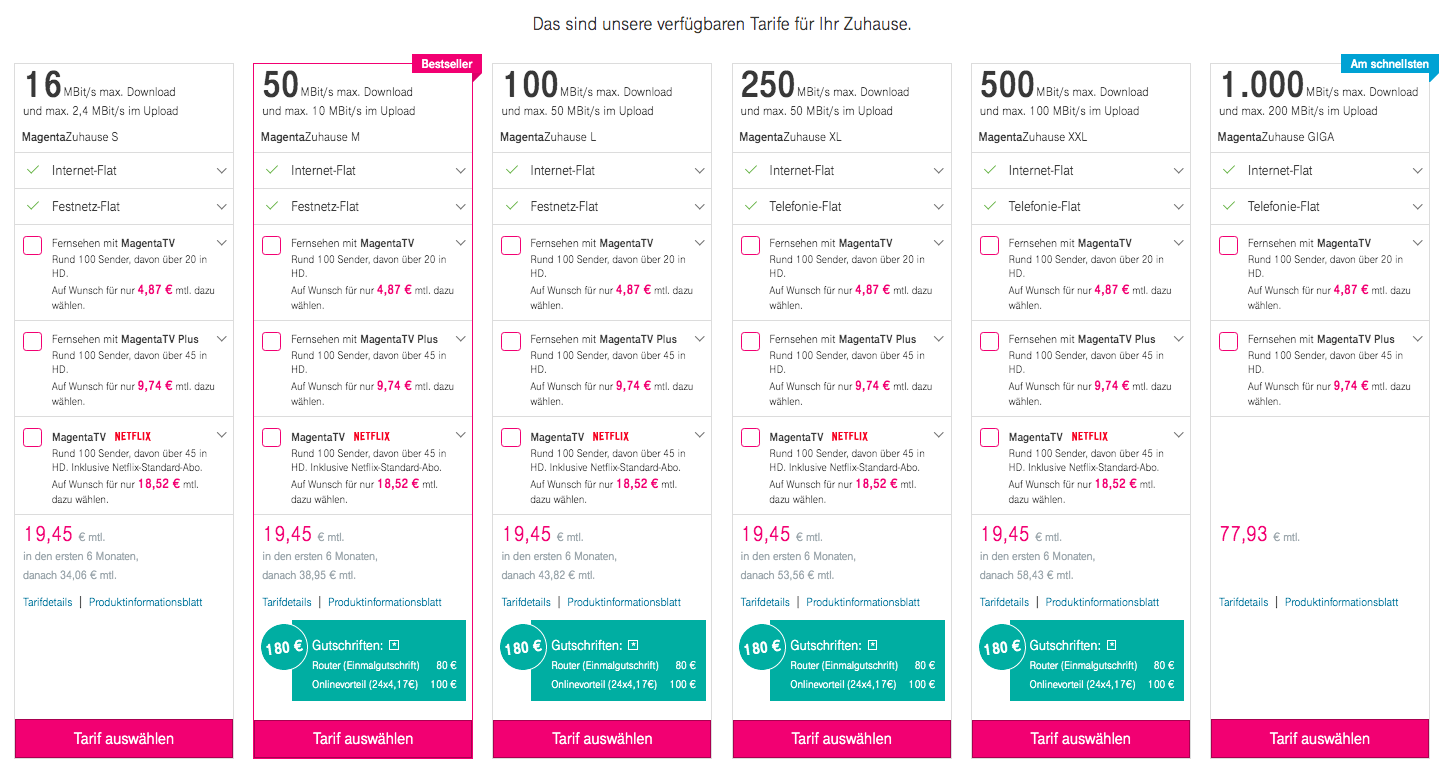
\includegraphics[scale=0.35]{./pictures/t-dsl.png}
\end{center}

{\vspace{-0.7cm}}
\begin{center}
  \textbf{Vodafone Tarif-Übersicht} \\
  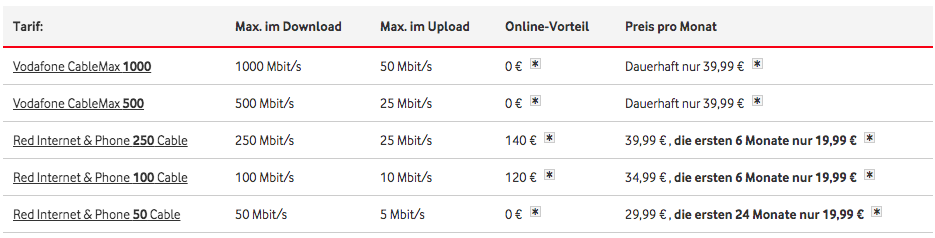
\includegraphics[scale=0.54]{./pictures/vodafoneKabel.png}
\end{center}

Die Telekom hat bei den Tarifen 250, 500, 1000 kürzlich den Upload reduziert, aber den Preis teils deutlich gesenkt.\\




  {\vspace{-0.4cm}}
  \begin{table}[ht]
    \begin{center}
    % \caption{alte Telekom Tarife}
    \label{alte Telekom Tarife}
    \begin{tabular}{|>{\raggedleft}p{3.5cm}| >{\centering}p{1cm}| >{\centering}p{1cm}| >{\centering}p{1cm}|}
      \hline
      \multicolumn{4}{|c|}{Frühere Datenraten} \tabularnewline \hline
      Download in Mbit/s & 250 & 500 & 1000 \tabularnewline
      \hline
      Upload in Mbit/s & 100 & 200 & 400 \tabularnewline \hline
    \end{tabular}
    \end{center}
  \end{table}

% \clearpage

\newpage

% \begin{minipage}


\begin{table}[ht]
  {\vspace{-1.5cm}}
  \begin{center}
    \textbf{Leistungsbeschreibungen der verschiedenen Tarife.}
  \end{center}
  \begin{center}
  % \caption{alte Telekom Tarife}
  \label{alte Telekom Tarife}
  \begin{tabular}{>{\centering}p{0.5\textwidth} >{\centering}p{0.5\textwidth}}
        \textbf{DSL 16} \\ 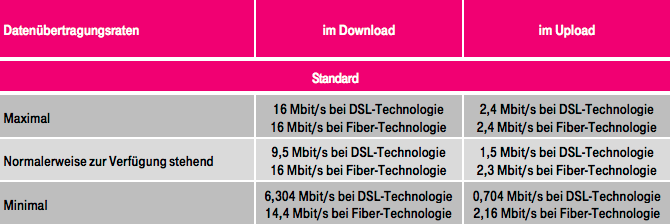
\includegraphics[width=0.5\textwidth, height=3cm]{./pictures/dsl16vertrag.png} & \textbf{DSL 50} \\ 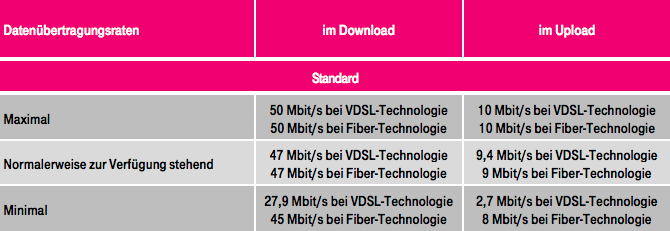
\includegraphics[width=0.5\textwidth, height=3cm]{./pictures/dsl50vertrag.png} \tabularnewline
        \textbf{DSL 100} \\ 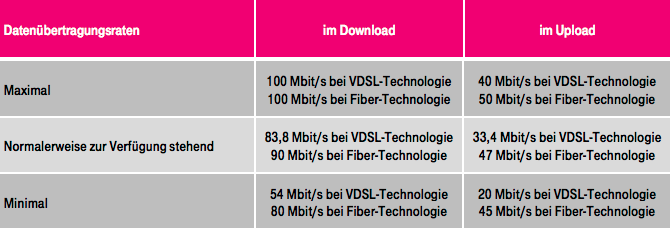
\includegraphics[width=0.5\textwidth, height=3cm]{./pictures/dsl100vertrag.png} & \textbf{DSL 250} \\ 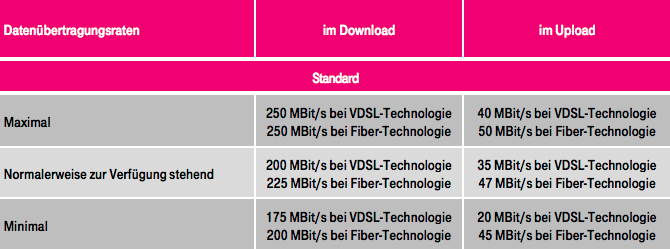
\includegraphics[width=0.5\textwidth, height=3cm]{./pictures/dsl250vertrag.png} \tabularnewline
        \textbf{DSL 500} \\ 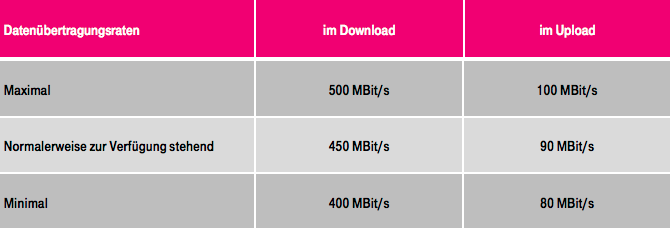
\includegraphics[width=0.5\textwidth, height=3cm]{./pictures/dsl500vertrag.png} & \textbf{DSL 1000} \\ 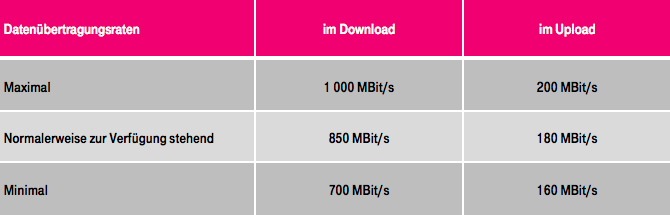
\includegraphics[width=0.5\textwidth, height=3cm]{./pictures/dsl1000vertrag.png} \tabularnewline
        &  \tabularnewline
        &  \tabularnewline
        \textbf{cable 50} \\ 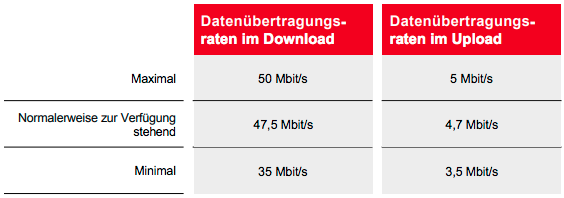
\includegraphics[width=0.5\textwidth, height=3cm]{./pictures/voda50.png} & \textbf{cable 100} \\ 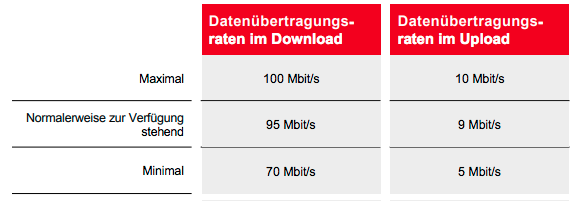
\includegraphics[width=0.5\textwidth, height=3cm]{./pictures/voda100.png} \tabularnewline
        \textbf{cable 250} \\ 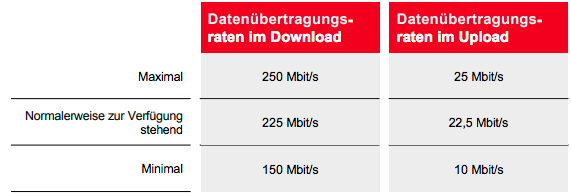
\includegraphics[width=0.5\textwidth, height=3cm]{./pictures/voda250.png} & \textbf{cable 500} \\ 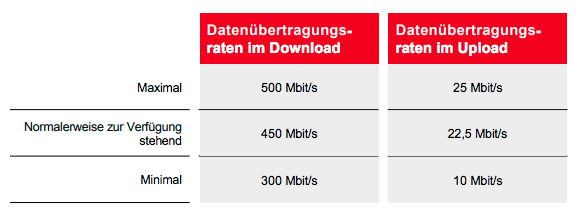
\includegraphics[width=0.5\textwidth, height=3cm]{./pictures/voda500.png} \tabularnewline
        \textbf{cable 1000} \\ 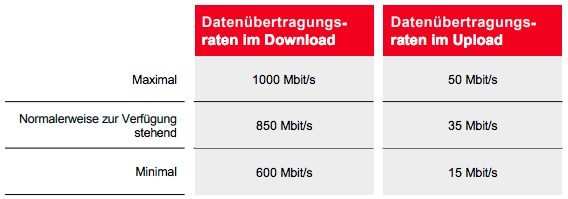
\includegraphics[width=0.5\textwidth, height=3cm]{./pictures/voda1000.png} &  \tabularnewline
  \end{tabular}
  \end{center}
\end{table}
\clearpage

% \begin{table}[ht]
%   {\vspace{-2cm}}
%   \begin{center}
%   % \caption{alte Telekom Tarife}
%   \label{alte Telekom Tarife}
%   \begin{tabular}{>{\centering}p{0.5\textwidth} >{\centering}p{0.5\textwidth}}
%         \textbf{DSL 16} 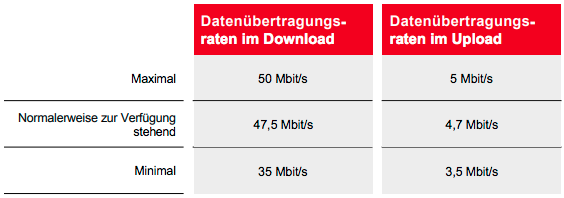
\includegraphics[width=0.4\textwidth, height=2.4cm]{./pictures/voda50.png} & \textbf{DSL 50} 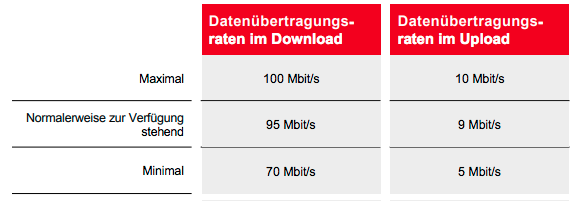
\includegraphics[width=0.4\textwidth, height=2.4cm]{./pictures/voda100.png} \tabularnewline
%         \textbf{DSL 100} 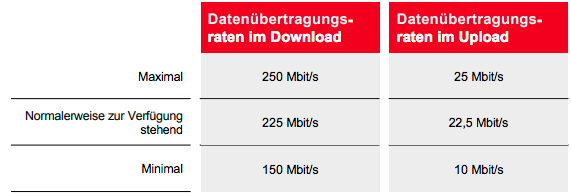
\includegraphics[width=0.4\textwidth, height=2.4cm]{./pictures/voda250.png} & \textbf{DSL 250} 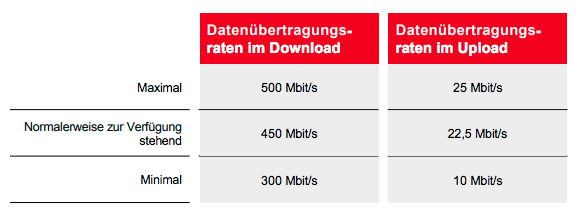
\includegraphics[width=0.4\textwidth, height=2.4cm]{./pictures/voda500.png} \tabularnewline
%         \textbf{DSL 500} 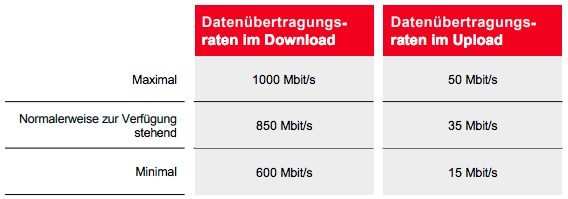
\includegraphics[width=0.4\textwidth, height=2.4cm]{./pictures/voda1000.png} &  \tabularnewline
%   \end{tabular}
%   \end{center}
% \end{table}
% \end{minipage}
% {\vspace{-0.7cm}}
% \begin{center}
%   \textbf{Vodafone Tarif-Übersicht} \\
%   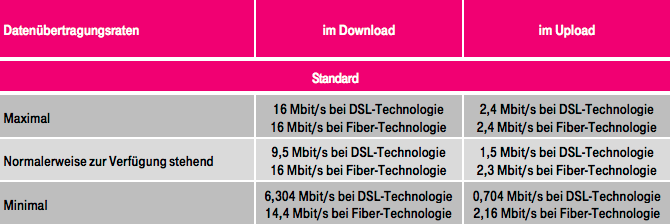
\includegraphics[scale=0.54]{./pictures/dsl16vertrag.png}
% \end{center}

\newpage
\subsub{Übersicht über die eigene Internetverbindung}

Zu Hause habe ich aktuell den kleinsten Telekom Vertrag, welcher aber mit 13€ für Internet + Telefon sehr günstig ist.
Von daher halten sich hier die Streaming-Möglichkeiten in Grenzen. \\
Da die Hochschule ans DFN angeschlossen ist und einen redundant synchronen 1 Gigabit Anschluss hat sind dort prinzipiell perfekte Streamingvoraussetzungen gegeben. Aber auch hier muss man beachten das diese nicht überall verfügbar sind. So übertragen die Wlan Router oft nur 600 Mbit/s im 2,4 GHz und 5 GHz Band und es ist ein geteiltes Medium, das heisst die Bandbreite steht einem nicht exclusiv zur Verfügung.

Relevant für Liveübertragungen ist hierbei der Upload welcher die maximal erreichbare Bildauflösung und Bildqualität beeinflusst.


\small
\color{black}
\vspace{0.3cm}
\begin{center}
  \begin{tikzpicture}
    \clip node (m) [matrix,matrix of nodes,
    fill=fulda_green!20,inner sep=0pt,
    nodes in empty cells,
    nodes={minimum height=1cm,minimum width=2.6cm,anchor=center,outer sep=0,font=\sffamily},
    row 1/.style={nodes={fill=fulda_green,text=white}},
    column 1/.style={nodes={fill=fulda_green,text=white,align=left,text width=3cm,text depth=0.5ex}},
    column 2/.style={text width=12cm,align=left,every even row/.style={nodes={fill=white}}},
    column 3/.style={text width=3cm,align=center,every even row/.style={nodes={fill=white}},},
    row 1 column 1/.style={nodes={fill=fulda_green}},%									1. spalte oben
    prefix after command={[rounded corners=4mm] (m.north east) rectangle (m.south west)}
    ] {
    & $\ \ $ T-DSL 16.0000 Fiber to the Curb\\
    $\ \ $ Download   	  & $\ \ $ 14,4 Mbit/s \\
    $\ \ $ Upload 				& $\ \ $ 2,16 Mbit/s \\
    };
  \end{tikzpicture}
\end{center}
\normalsize

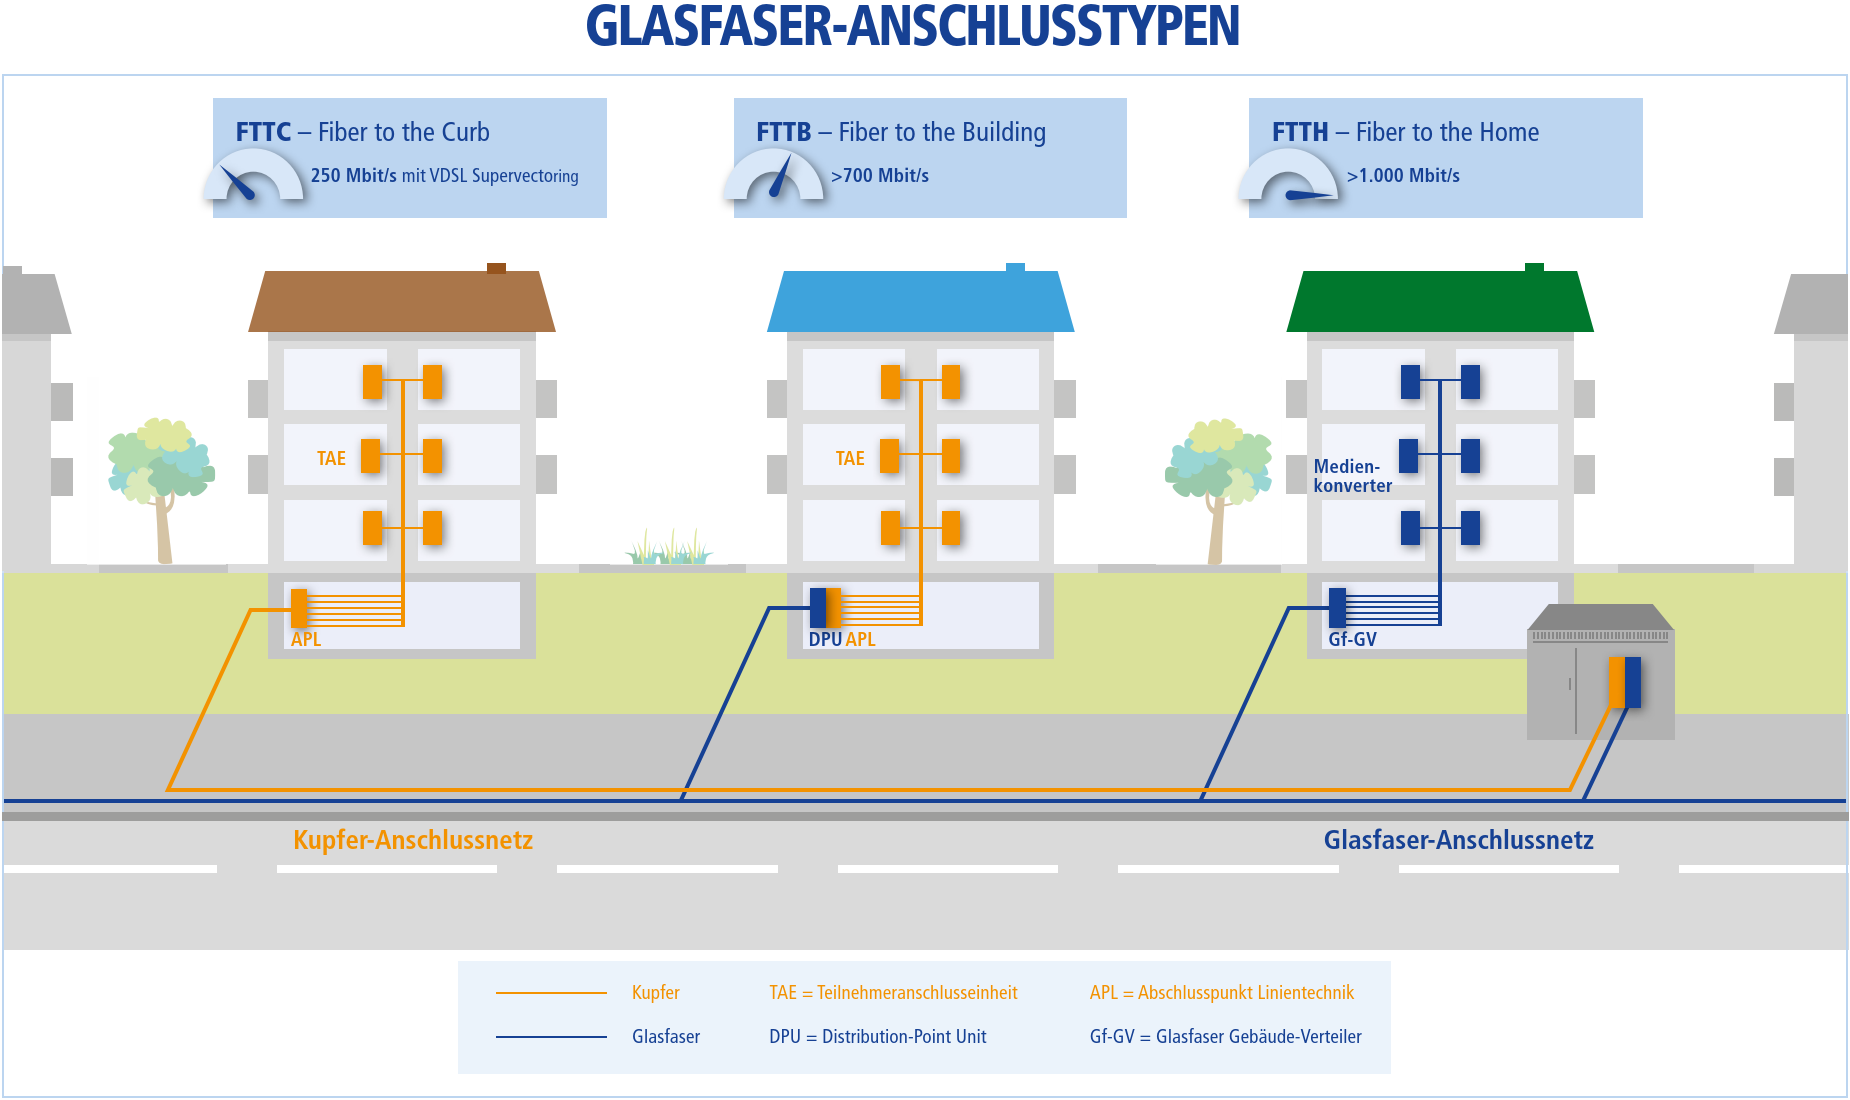
\includegraphics[width=\textwidth]{./pictures/fttc.png}

{\vspace{0.5cm}}

Der Internetanschluss wird über  \quote{Fiber to the curb} bereitgestellt. Hierfür wurden von der Rhön Energie Glasfaser-Leitungen bis in den Verteilerkasten gelegt. Die letzte Meile wird über Kupfer übertragen, welches seit ein paar Monaten nun auch mit VDSL2 geschieht. Dadurch sind nun Datenraten bis 250Mbit im Download verfügbar. Aber weil die Telekom den Upload halbiert hat ist dieser Tarif aber grade fürs Streaming unintressanter geworden. \\

50 Mbit/s im Upload wären prinzipiell aber trotzdem für alle Streaming-Auflösungen und fast alle Datenraten ausreichend.



\subsub{Überprüfen des Heimnetzes}
% \subsub{Überprüfen der Internetverbindung}

Für das Überprüfen der Internetverbindung muss man erst mal alle Störungen im Heimnetz ausgeschlossen haben. Der einfachste Weg ist ein direkt verbundenes fertig konfektioniertes Netzwerkkabel zwischen dem PC und dem Internetrouter. Da die Netzwerkkarte am Hackintosh (Eigenbau PC auf welchem MacOS läuft) wegen des schlechten Treiber recht instabil läuft verwende ich für alle Datenübertragungen Wlan.\\
Bei der Nutzung von Wlan ist darauf zu achten das ein möglichst nicht von einem anderen Wlan-Router genutzten Kanal verwendet wird. Wenn sich Wlan-Netzwerke überschneiden wie unten im Bild beim 2,4 GHz Band dann kann es zu Einbusen kommen wenn bei Router viele Daten übertragen. Das Wlan über die AVM Fritzbox wurde nur für dieses Foto aktiviert, da dieses bei der Fritzbox Wlan 7490 dermaßen schlecht ist, sodass es in der Regel nur sehr eingeschränkt nutzbar ist.
Da ich auf dem Land in einer Souterrain-Wohnung lebe, welche vor dem Fenster zusätzlich gut bepflanzt ist, werden die Wlan-Router der Nachbarn komplett abgeschirmt.\\


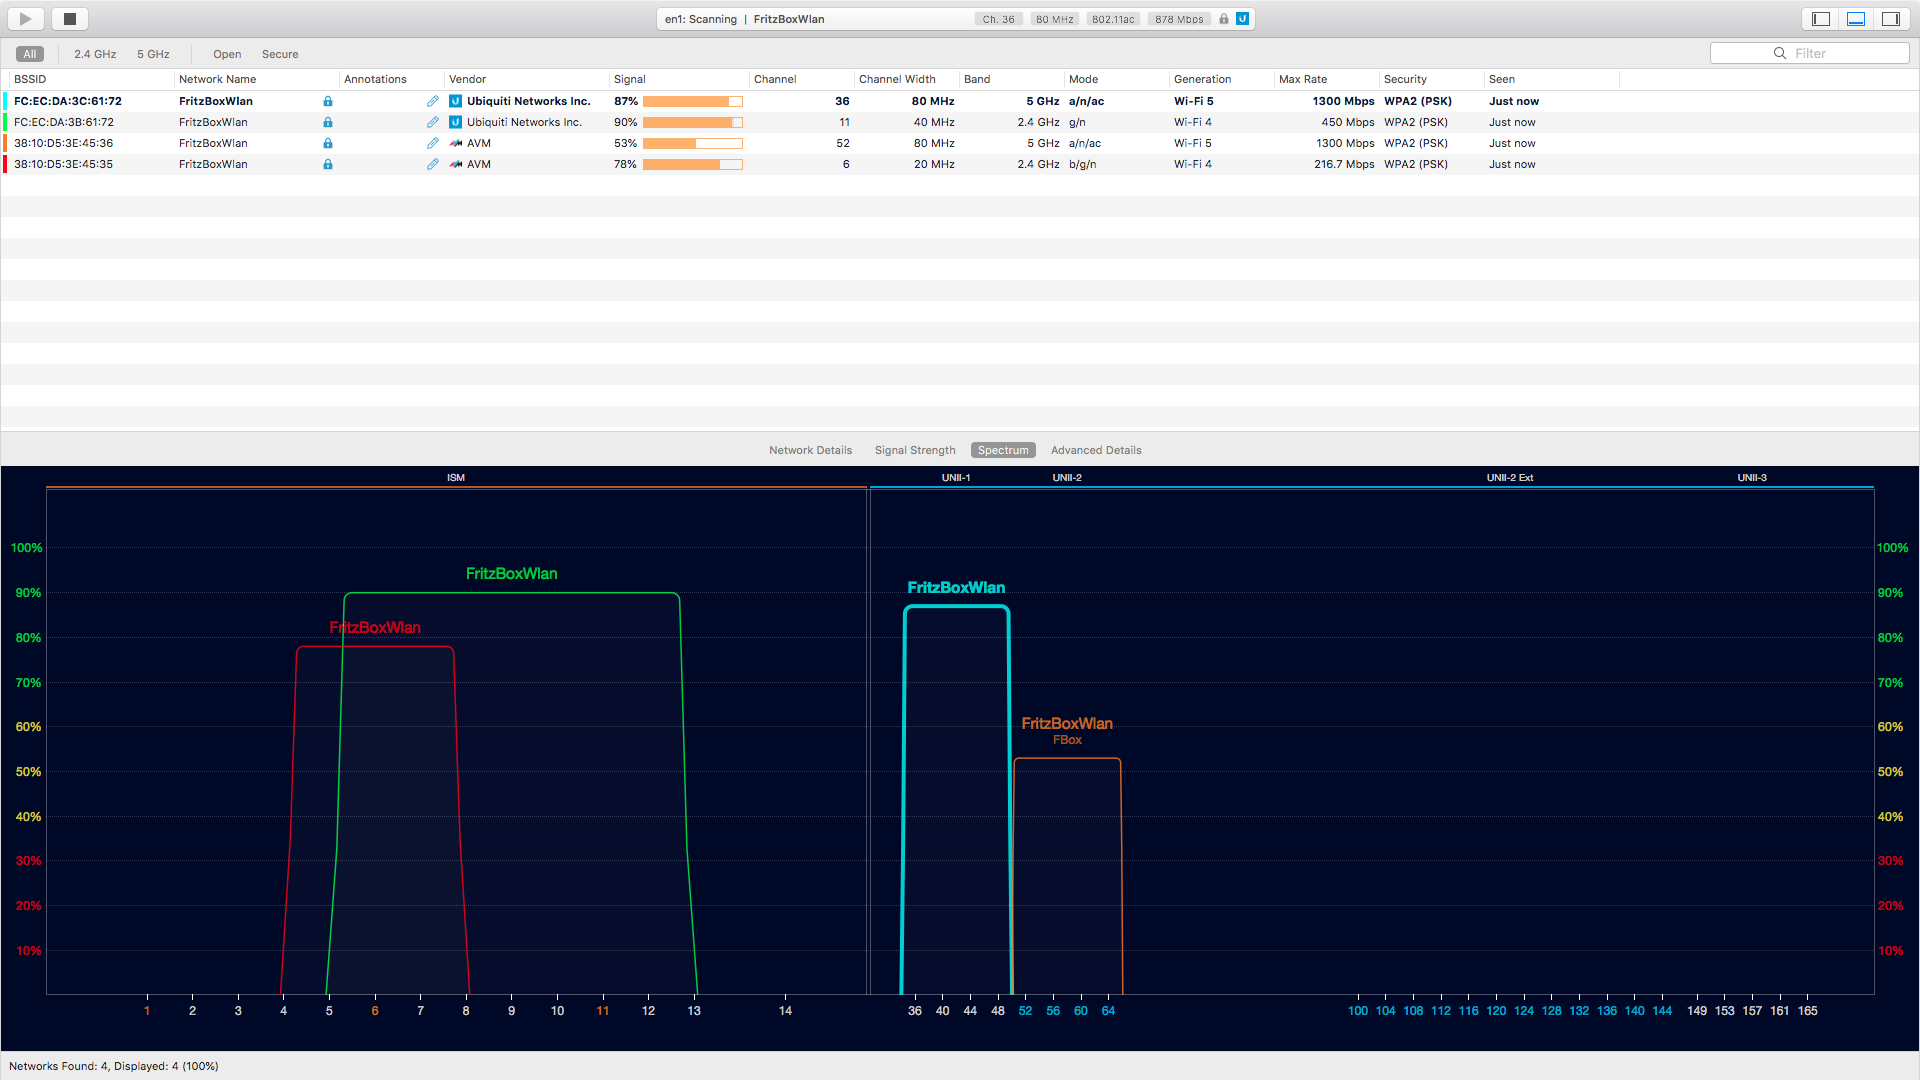
\includegraphics[width=\textwidth]{./pictures/wifiNetworks.png}

Des weiteren sollte man kontrollieren ob nicht irgendwo im Netzwerk irgendwelche Stromsparfunktionen aktiv sind.

{\vspace{0.2cm}}
\begin{center}
  % \textbf{DSL-Informationen der FritzBox} (ADSL 2+ = VDSL)\\
  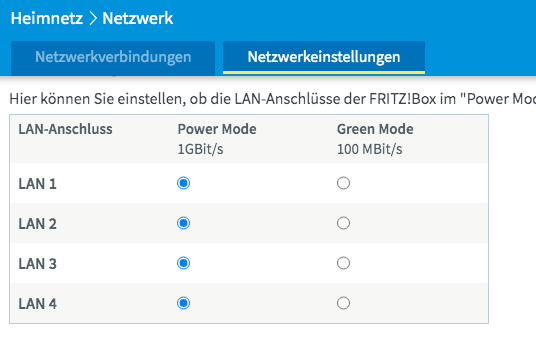
\includegraphics[scale=0.40]{./pictures/powerSaveNetwork.png}
\end{center}

Durch magnetische Felder und andere Störungen im Haus kann es aber vorkommen, \\
dass die Netzwerkgeräte die Gigabitverbindung nicht synchronisiert bekommen.
Dann fallen diese beispielsweise auf 100 Megibit oder im schlimmsten Fall auch auf 10 Megabit zurück.
% {\vspace{0.2cm}}
\begin{center}
  % \textbf{DSL-Informationen der FritzBox} (ADSL 2+ = VDSL)\\
  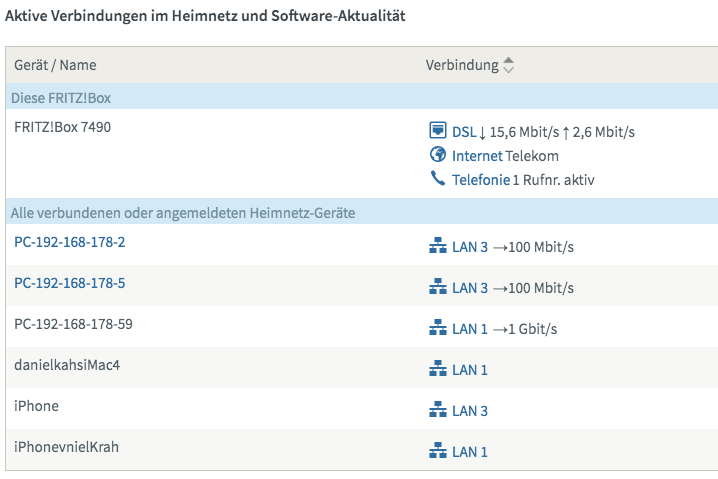
\includegraphics[scale=0.40]{./pictures/aktuelleNetzwerkGeraete.png}
\end{center}

Das ist beispielsweise beim Lan-Anschluss 3 der Fall. Hier führt ein selbst konfektioniertes Kabel mit 60 Metern parallel mit 4 Satkabeln durch mehrere Kellerräume in den Dachboden zu 2 weiteren Wlan-Routern. Diese können zwar prinzipiell 1 Gigabit/s übertragen, können aber nicht erfolgreich synchronisieren was für deren Nutzung/Funktion aber keine Rolle spielt. \\

\quote{PC-192-168-178-59} ist der Ubiquity Unify AC Pro welcher das Wlan im genutzten Zimmer bereit stellt.

% {\vspace{0.2cm}}
\begin{center}
  % \textbf{DSL-Informationen der FritzBox} (ADSL 2+ = VDSL)\\
  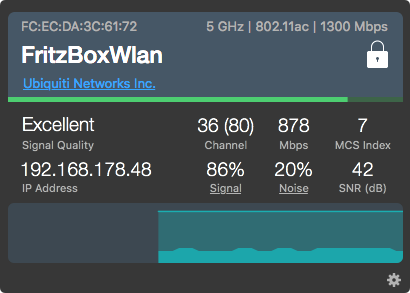
\includegraphics[scale=0.5]{./pictures/wlanSynced.png}
\end{center}

Synchronisiert wird bei 1300 Mbit/s und es stehen leicht schwankend ca. 878 Mbit/s für Nutzdaten zur Verfügung.
Von daher ist hier auch nicht mit Engpässen zu rechnen.


\newpage
\subsub{Überprüfen der Verbindung zwischen DSL-Router und Vermittlungsstelle}

Wenn eine fehlerfreie Verbindung zum Router sichergestellt ist folgt als nächstes die Überprüfung und Konfiguration der Verbindung zwischen Router und Vermittlungsstelle. \\

{\vspace{-0.1cm}}
\begin{center}
  \textbf{DSL-Informationen der FritzBox} (ADSL 2+ = VDSL)\\
  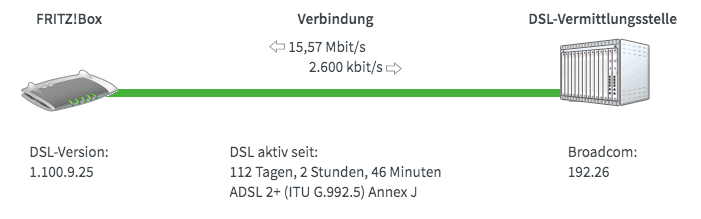
\includegraphics[scale=0.50]{./pictures/dslinfo.png}
\end{center}
Das entspricht in etwa dem gebuchten Tarif ist also ok.\\

{\vspace{-0.1cm}}
\begin{center}
  \textbf{Einstellen der Fehlerkorrektur (Störsicherheit)}\\
  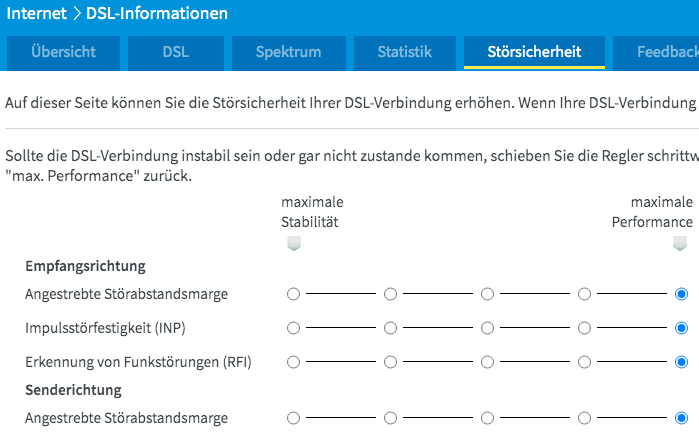
\includegraphics[width=\textwidth]{./pictures/stoersicherheit.png}
\end{center}
% 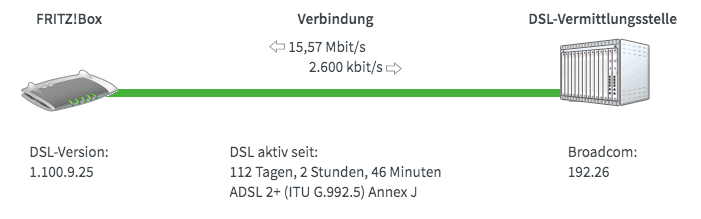
\includegraphics[width=\textwidth]{./pictures/dslinfo.png}

\newpage

Für Streaming ist es wichtig das die Daten in Echtzeit übertragen werden.
Wenn Übertragungsfehler auftreten ergibt es bei Live-Streaming keinen Sinn die Daten erneut zu senden.


{\vspace{-0.1cm}}
\begin{center}
  \textbf{Verbindungs-Informationen}\\
  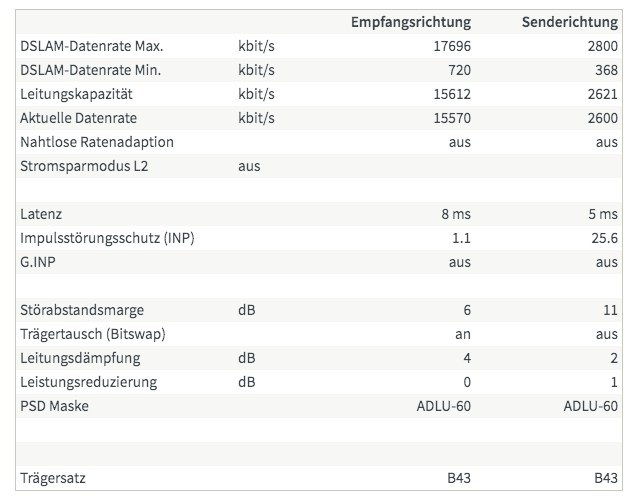
\includegraphics[scale=0.50]{./pictures/leitungsinformation.png}
\end{center}

{\vspace{-0.1cm}}
\begin{center}
  \textbf{Übertragungsfehler-Informationen}\\
  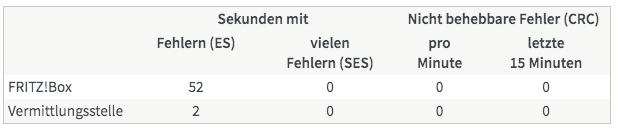
\includegraphics[scale=0.50]{./pictures/leitungsinformationFehler.png}
\end{center}

54 Fehler in 112 Tagen kann man vernachlässigen. Sollten diese innerhalb von Minuten hoch zählen sollte man die Regler nach links verschieben.
Dies drosselt dann die Verbindung wie beim Heimnetz herunter. Hier muss man das aber manuell tun und geschieht nicht automatisch.\\

Nun kann man eine zufällige Verbindung zu einem Server z.B über \quote{speedtest.net} im Internet testen.
\begin{center}
  \textbf{Ergebnis des Geschwindigkeitstest mittels Webseite} \\
  {\vspace{0.3cm}}
  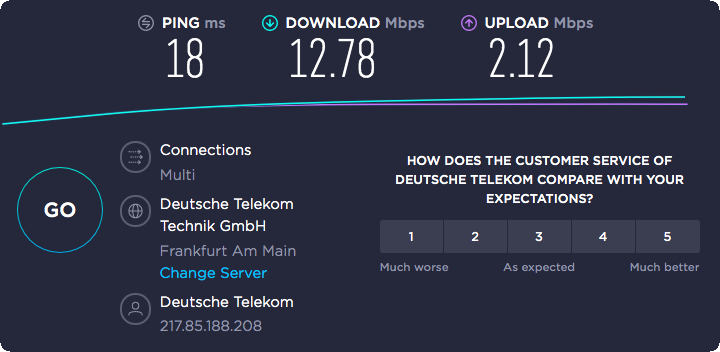
\includegraphics[scale=0.45]{./pictures/speedtestWeb.png}
\end{center}

Das entspricht dem was einem die Telekom in der Leistungsbeschreibung minimal garantiert.

Als Gegenprobe kann man den Test auch noch über das Terminal ausführen. \\

\monocodebox{sh}{Speedtest mittels Terminal:}{./codesnippets/speedtest.sh}{false}{0}{9999999}

Hier wurden ähnliche Ergebnisse erreicht, man sollte also 12 Mbit/s im Download und 2 Mbit im Upload als gegeben ansehen.



\subsub{Streaming über Youtube}

Youtube gibt, als Voraussetzung beim streamen mit einem Mobiltelefon, an das ein Stream etwa 10MB pro Minute verbraucht. \\
Eine Angabe bei welcher Auflösung und Bitrate dies der Fall ist sucht man vergebens. \\

\begin{tcolorbox}[colback=fulda_green!50!white,colframe=fulda_green,title=Berechnung der benötigten Datenrate]
  10MB * 8 (bit) : 60 (Sekunden)= \textasciitilde 13,3 Mbit/s
\end{tcolorbox}
Wenn man per Handy streamt wird ein Stromverbrauch vom 1\% pro Minute angegeben. Auch hier wird nicht darauf einegangen welches Mobiltelefon verwendet wird.
Also muss man sich sinnvolle Werte selber aus weiteren Quellen suchen oder selbst ausloten. \\

Erwünschenswert für ein Filmfestival ist eine Auflösung von 1080p. \\
Prinzipiell reichen hier 30 Bilder pro Sekunde aus, je nach Film können aber auch 60 Bilder von Vorteil sein. \\
So senden die öffentlich rechtlichen Sender wie ARD und ZDF in 720p50 da hier 50 Vollbilder pro Sekunde möglich sind. Die Sendeanstalten begründen diese Wahl damit, dass diese Auflösungs/Bildwiederholfrequenz Kombination insbesondere bei Sportveranstaltungen, bei denen schnelle Bewegungen vorkommen, von Vorteil ist.\\
Ansonsten könnten Sie nur in 1080i senden, welches über Satellit nur mit 24 oder 30 Vollbildern, sowie 60 Halbbildern im Zeilensprungverfahren möglich ist.
Man spart, mit ca 46,1 Mpx/s im Gegensatz zu 62,2 Mpx/s bei 1080p30/i60, auch etwas an Daten welche übertragen werden müssen.\\

Bei der Übertragung über das Internet spielt dies bei einer Flatrate aber keine Rolle. \\
Außer man streamed über seinen Mobilfunkvertrag oder beispielsweise über das Netz der Universität Darmstadt, da diese nicht am DFN hängen und für ihren Datenverkehr bezahlen müssen.

\subsub{Welche Datenrate wird bei welcher Auflösung benötigt?}

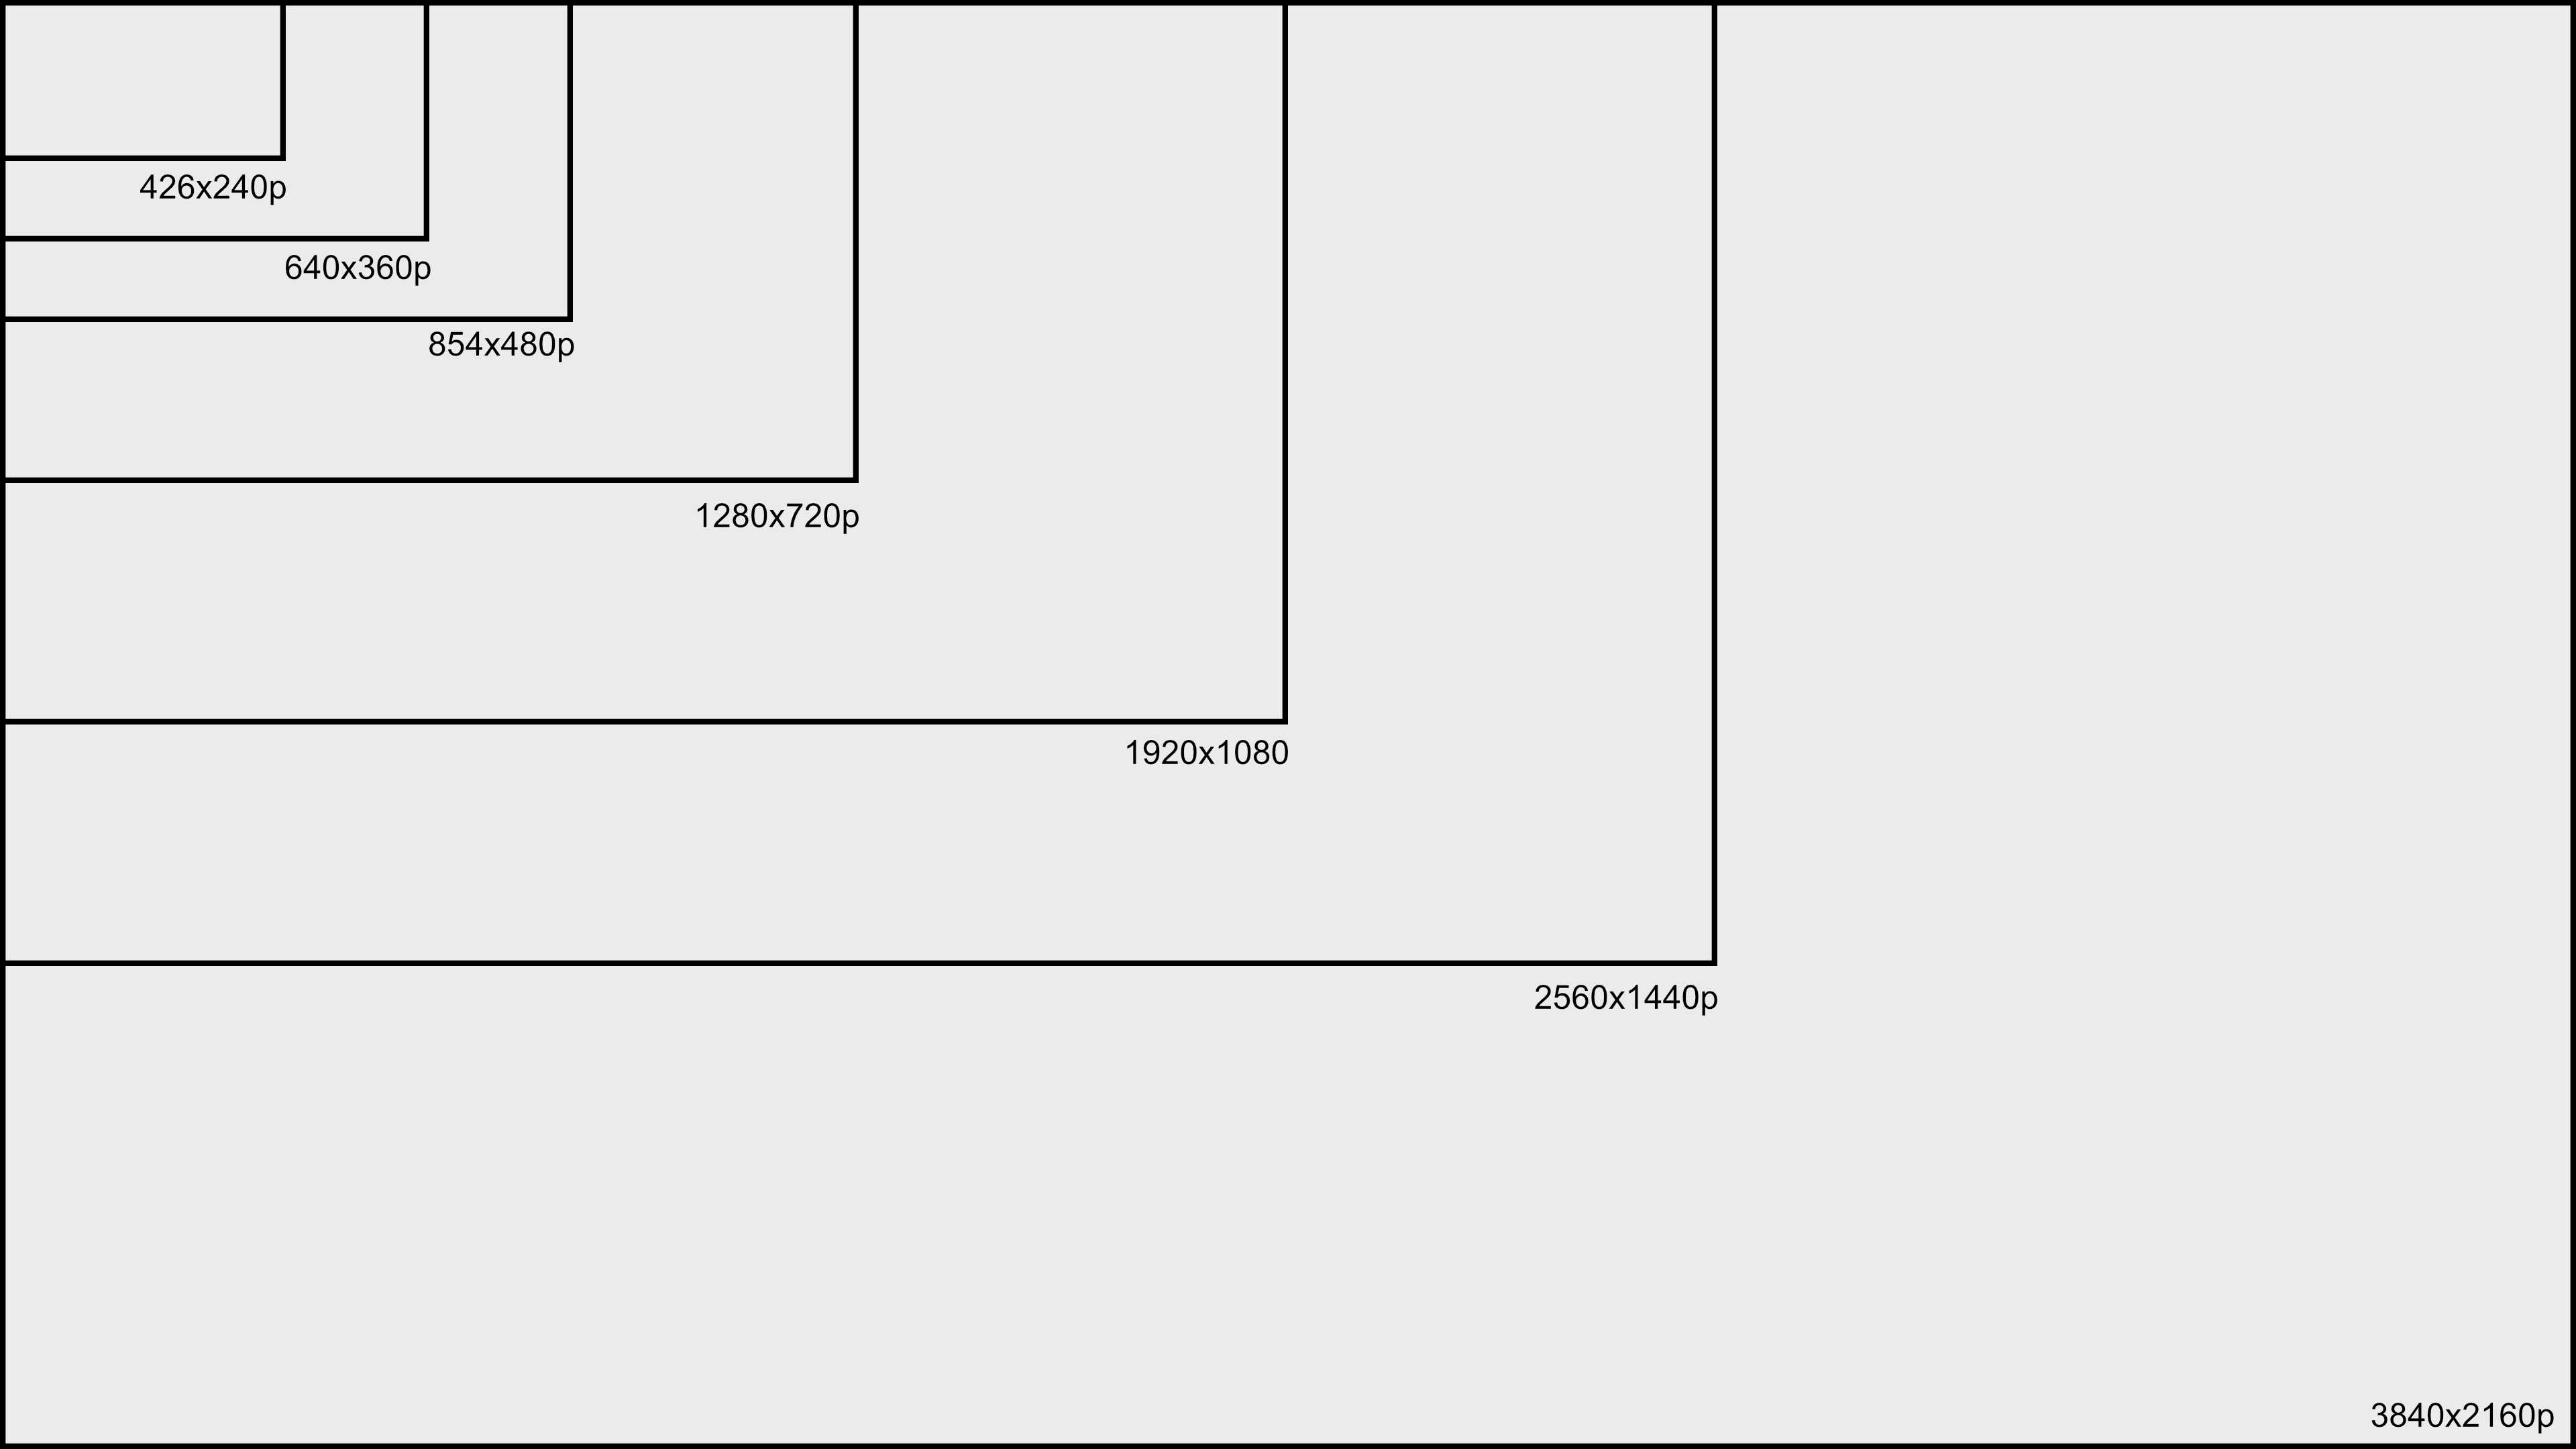
\includegraphics[width=\textwidth]{./pictures/resolutions.png}

\begin{center}
  \textbf{Empfohlene Datenraten für Youtube}
  \begin{table}[ht]
    \begin{tabular}{|>{\raggedleft}p{1,6cm} >{\raggedleft}p{1,9cm}| >{\centering}p{1,4cm}| >{\raggedleft}p{0,9cm}>{\raggedleft}p{0,1cm} >{\raggedleft}p{2,07cm}|  >{\centering}p{2,3cm}| >{\centering}p{2,8cm}|}   % \begin{tabular}*{5}{|c}      %
      \hline
      \rowcolor{fulda_green}
      \multicolumn{2}{|c|}{Auflösung}   &  Bildrate     & \multicolumn{3}{|c|}{Video-Bitrate in kbit/s}         &  Audio-Bitrate    & Minimaler Upload Mbit   \tabularnewline  \hline  \hline  \rowcolor{fulda_green!66}
      4k/2160p  & 3.840x2.160p          & 60            & 20.000 & – & 51.000 kbit/s    & 128 kbits/s       & 40.2 Mbit/s            \tabularnewline  \hline  \rowcolor{fulda_green!33}
      4k/2160p  & 3.840x2.160p          & 30            & 13.000 & – & 34.000 kbit/s    & 128 kbits/s       & 26.2 Mbit/s            \tabularnewline  \hline  \rowcolor{fulda_green!66}
      1440p     & 2.560x1.440p          & 60            & 9.000 & – & 18.000 kbit/s     & 128 kbits/s       & 18.2 Mbit/s            \tabularnewline  \hline \rowcolor{fulda_green!33}
      1440p     & 2.560x1.440p          & 30            & 6.000 & – & 13.000 kbit/s     & 128 kbits/s       & 12.2 Mbit/s            \tabularnewline  \hline  \rowcolor{fulda_green!66}
      1080p     & 1.920x1.080p          & 60            & 4.500 & – & 9.000 kbit/s      & 128 kbits/s       & 9.2 Mbit/s             \tabularnewline  \hline \rowcolor{fulda_green!33}
      1080p     & 1.920x1.080p          & 30            & 3.000 & – & 6.000 kbit/s      & 128 kbits/s       & 6.2 Mbit/s             \tabularnewline  \hline  \rowcolor{fulda_green!66}
      720p      & 1.280x720p            & 60            & 2.250 & – & 6.000 kbit/s      & 128 kbits/s       & 4.7 Mbit/s             \tabularnewline  \hline \rowcolor{fulda_green!33}
      720p      & 1.280x720p            & 30            & 1.500 & – & 4.000 kbit/s      & 128 kbits/s       & 3.2 Mbit/s             \tabularnewline  \hline  \rowcolor{fulda_green!66}
      480p      & 854x480p              & 30            & 500 & – & 2.000 kbit/s        & 128 kbits/s       & 1.2 Mbit/s             \tabularnewline  \hline \rowcolor{fulda_green!33}
      360p      & 640x360p              & 30            & 400 & – & 1.000 kbit/s        & 128 kbits/s       & 1 Mbit/s               \tabularnewline  \hline  \rowcolor{fulda_green!66}
      240p      & 426x240p              & 30            &  300 & – & 700 kbit/s         & 128 kbits/s       & 0.8 Mbit/s              \tabularnewline  \hline \rowcolor{fulda_green!33}
    \end{tabular}
  \end{table}
\end{center}

Im oberen Bild sieht man einen Größenvergleich der einzelnen Videoauflösungen. In der unteren Tabelle sind empfohlene Datenraten basierend aus Informationen verschiedenster Foren sowie sozialer Netzwerke. \\

Bei der Videobitrate ist der Minimalwert immer so hoch damit das Bild eine akzeptable Qualität hat. Beim Maximalwert ist kein Qualitätsverlust sichtbar.
Da es bei der Datenübertragung immer zu Schwankungen kommen kann, beispielsweise wenn: \quote{Abends alle Netflix schauen} , sollte man einen Puffer einplanen. Pi mal Daumen nimmt man die minimale Datenrate mal 2 und addiert die Tondatenrate, aufgerundet auf die nächste 100er Stelle, auf. \\

\newpage
So kann, es wie man sieht, bei einem DSL 50 Vertrag über Fiber bei 1080p60 \\
schon knapp werden. Im schlimmsten Fall steht man beim Upload nicht viel besser da als mit meinem DSL 16 Vertrag, wenn der Upload komplett über die störungsanfälligere VDSL Technologie übertragen wird und nicht wie bei Fiber to the curb, zumindest auf einer Teilstrecke, über Glasfaser. \\

Während man so über FTTC relativ sicher kalkulieren kann, sollte man bei reiner VDSL Technik für 1080p mindestens DSL 100 buchen.\\

1440p60 sollte über Kupfer VDSL grade so noch gehen, für 4K Streams benötigt aber mindestens FTTC mit DSL 100 oder besser einen direkten Glasfaseranschluss.


\subsub{Latenz}

Wenn man eine Moderation und/oder Livechat nutzen möchte, sollte man sich auch mit den Latenzen beschäftigen.

So empfehlen einige Youtuber für 1080p-Streams:
\begin{itemize}
  \item Normale Latenz: \textasciitilde 6-10 Mbit/s
  \item Niedrige Latenz: \textasciitilde 5-6 Mbit/s
  \item Sehr niedrige Latenz: \textasciitilde 4,5-5 Mbit/s
\end{itemize}

Letztere ist wichtig wenn man Echtzeitkommunikation mit den Zuschauern halten möchte, ansonsten kann es zu Verzögerungen von 5 Sekunden und auch deutlich mehr im Chat kommen.

\subsub{Exkurs zu anderen Plattformen}

Bei Twitch kann man wenn man nicht Twitch-Partner ist langfristig höchstens mit 720p und einer Datenrate von 3-3,5 Mbit/s streamen.

Bei anderen Webseiten welche Livestreaming anbieten sieht es ähnlich aus.\\
Facebook (720P @ \textasciitilde 4 Mbit/s) \\
Mixer (720P @ \textasciitilde 6 Mbit/s) \\

Twitch und Mixer unterstützen, wenn man kein Partner ist, kein downscaling.
Das bedeutet das wenn man auf seinem Mobiltelefon und LTE einen Stream schauen möchte, nur 720p zur Verfügung hat und nicht auf 360p umschwenken kann um sein Datenvolumen zu schonen. \\

Mixer, welcher ein Dienst von Microsoft war, wurde am 23. Juli 2020 geschlossen.


\newpage
